\section*{Problem 5}
\begin{enumerate} [(a)]
	\item \begin{proof} [Solution]
		\mbox{}\\
		\begin{center}
			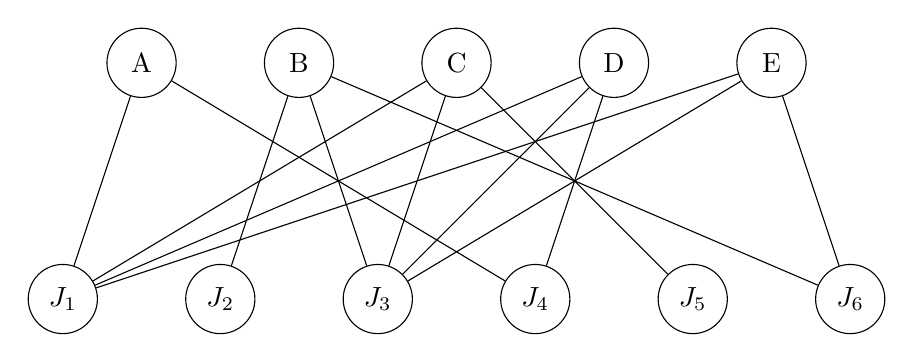
\begin{tikzpicture}
				\tikzstyle{Vertex} = [circle, draw, minimum size=25, inner sep=0pt]	
				\node (A) at (0,3) [Vertex, fill=white] {A};
				\node (B) at (2,3) [Vertex, fill=white] {B};
				\node (C) at (4,3) [Vertex, fill=white] {C};
				\node (D) at (6,3) [Vertex, fill=white] {D};
				\node (E) at (8,3) [Vertex, fill=white] {E};
				\node (J1) at (-1,0) [Vertex, fill=white] {$J_1$};
				\node (J2) at (1,0) [Vertex, fill=white] {$J_2$};
				\node (J3) at (3,0) [Vertex, fill=white] {$J_3$};
				\node (J4) at (5,0) [Vertex, fill=white] {$J_4$};
				\node (J5) at (7,0) [Vertex, fill=white] {$J_5$};
				\node (J6) at (9,0) [Vertex, fill=white] {$J_6$};
				\draw [-] (A) to (J1);
				\draw [-] (A) to (J4);
				\draw [-] (B) to (J2);
				\draw [-] (B) to (J3);
				\draw [-] (B) to (J6);
				\draw [-] (C) to (J1);
				\draw [-] (C) to (J3);
				\draw [-] (C) to (J5);
				\draw [-] (D) to (J1);
				\draw [-] (D) to (J3);
				\draw [-] (D) to (J4);
				\draw [-] (E) to (J1);
				\draw [-] (E) to (J3);
				\draw [-] (E) to (J6);
			\end{tikzpicture}
		\end{center}
	\end{proof}
	\item \begin{proof} [Solution]
		\mbox{}\\
		\begin{center}
			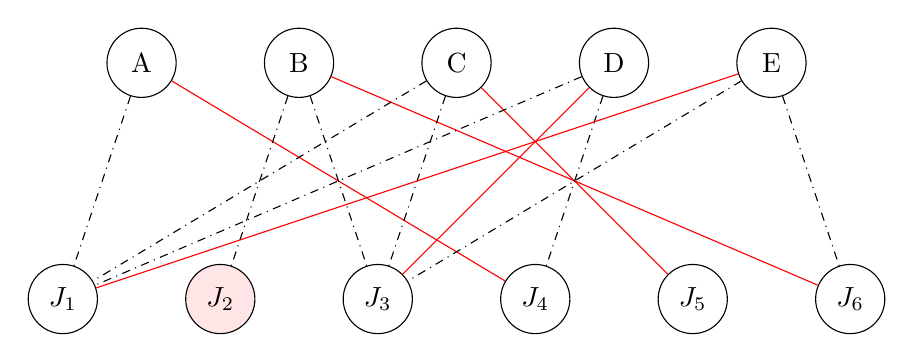
\begin{tikzpicture}
				\tikzstyle{Vertex} = [circle, draw, minimum size=25, inner sep=0pt]	
				\node (A) at (0,3) [Vertex, fill=white] {A};
				\node (B) at (2,3) [Vertex, fill=white] {B};
				\node (C) at (4,3) [Vertex, fill=white] {C};
				\node (D) at (6,3) [Vertex, fill=white] {D};
				\node (E) at (8,3) [Vertex, fill=white] {E};
				\node (J1) at (-1,0) [Vertex, fill=white] {$J_1$};
				\node (J2) at (1,0) [Vertex, fill=red, fill opacity=0.1, text opacity=1] {$J_2$};
				\node (J3) at (3,0) [Vertex, fill=white] {$J_3$};
				\node (J4) at (5,0) [Vertex, fill=white] {$J_4$};
				\node (J5) at (7,0) [Vertex, fill=white] {$J_5$};
				\node (J6) at (9,0) [Vertex, fill=white] {$J_6$};
				\draw[dash dot] [-] (A) to (J1);
				\draw[red] [-] (A) to (J4);
				\draw[dash dot] [-] (B) to (J2);
				\draw[dash dot] [-] (B) to (J3);
				\draw[red] [-] (B) to (J6);
				\draw[dash dot] [-] (C) to (J1);
				\draw[dash dot] [-] (C) to (J3);
				\draw[red] [-] (C) to (J5);
				\draw[dash dot] [-] (D) to (J1);
				\draw[red] [-] (D) to (J3);
				\draw[dash dot] [-] (D) to (J4);
				\draw[red] [-] (E) to (J1);
				\draw[dash dot] [-] (E) to (J3);
				\draw[dash dot] [-] (E) to (J6);
			\end{tikzpicture}
		\end{center}
	\end{proof}
	\item \begin{proof}
		We cannot make complete(perfect) matching. There are two theorems.
		\begin{itemize}
			\item If perfect matching exists, then it has even nodes.
			\item (\textit{Hall\textquotesingle s theorem}) Let bipartite $G = (V_1\cup V_2, E)$ be given. For $S\subseteq V_1$, define $N(S) = \{v \in V_2\mid v\mbox{ is adjecent to }u\in S\}$. Then there is a perfect matching if and only if $\left|S\right| \leq \left|N(S)\right|$ for $^\forall S\subseteq V_1$.
		\end{itemize}
		The above graph has total 11 nodes. Also, let $S = V_1 = \{J_1, J_2, \cdots, J_6\}$. Then $N(S) = V_2 = \{A, B, C, D, E\}$, so $\left|S\right| > \left|N(S)\right|$.\\
	\end{proof}
\end{enumerate}